%%%% utfpr-article.tex, 2025/08/07
%%%% Copyright (C) 2016-2025 Luiz E. M. Lima (luizeduardomlima@gmail.com)
%%
%% This work may be distributed and/or modified under the conditions of the
%% LaTeX Project Public License, either version 1.3 of this license or (at your
%% option) any later version.
%% The latest version of this license is in
%%   https://www.latex-project.org/lppl.txt
%% and version 1.3 or later is part of all distributions of LaTeX version
%% 2005/12/01 or later.
%%
%% This work has the LPPL maintenance status `maintained'.
%%
%% The Current Maintainer of this work is Luiz E. M. Lima.
%%
%% This work consists of all files listed in readme.html.
%%
%% A brief description of this work is in readme.txt.

%% Conformidade com PDF/A (LaTeX release 2022-06-01 or later)
% \DocumentMetadata{pdfstandard = A-3b, pdfversion = 1.7, lang = pt-BR}

%% Detecção e aviso sobre comandos obsoletos
% \RequirePackage[l2tabu, orthodox]{nag}

%% Classe de documento
\documentclass[%% Opções (^ = padrão; > = para pacotes):
  a4paper,%% Tamanho de papel: a4paper, letterpaper (^), etc.
  12pt,%% Tamanho de fonte: 10pt (^), 11pt ou 12pt
  fleqn,%% Alinhamento de equações à esquerda (centralizado por padrão)
%   draft,%% Aparência de documento (>): draft ou final (^)
  english,%% Idioma secundário (penúltimo) (>)
  brazilian,%% Idioma primário (último) (>)
]{article}

%% Pacotes utilizados
\usepackage[%% Opções (^ = padrão; ¹ = Leiaute A; ² = Leiaute B):
%   Layout    = A,%% Leiaute (margens): A (esquerda menor + recuo) ou B (iguais) (^)
%   Font      = Times,%% Fonte principal: Arial (²), Calibri (¹), Times ou LaTeX(*)
%   TextColor = 575757,%% Cor (HTML) texto (preto ^): cinzento
%   EmphColor = 008080,%% Cor (HTML) ênfase (preto ^): verde azulado
%   LinkColor =,%% Cor (HTML) hyperlink (azul escuro ^): nenhuma (cor texto)
%   Rule      = Both,%% Linha (cabeçalho e rodapé): None (²), Header, Footer ou Both (¹)
%   AffilIcon = Off,%% Ícones de e-mail, Lattes, ORCID e Instituição: On (^) ou Off
%   DocLic    = None,%% Licença do documento: CC (Creative Commons) (^) ou None
%   CCLic     = BY-NC-ND,%% Licença CC: BY (^), BY-SA, BY-ND, BY-NC, BY-NC-SA ou BY-NC-ND
%   PageNum   = Off,%% Numeração de páginas: On (^) ou Off
%   SectNum   = Off,%% Numeração de seções (\section): On (²) ou Off (¹)
%   UnnumSect = Center,%% Alinhamento de seções (\section*): Center (¹) ou Left (²)
%   Caption   = Left,%% Alinhamento de legendas: Center (^) ou Left
%   Source    = Left,%% Alinhamento de fontes (autoria): Center (^) ou Left
%   ABNTCit   = NSB,%% Citação ABNT: AAY (Nome, Ano) (^), NRB (1) ou NSB [1]
%   DOIIcon   = On,%% Ícone de DOI em referências: On ou Off (^)
%   URLIcon   = On,%% Ícone de URL em referências: On ou Off (^)
%   Index     = On,%% Índice Remissivo (makeindex): On ou Off (^)
]{utfpr-article}

%% Informações do documento (descomentar para alterar; * = opcional)
%%%% Título: [Cabeçalho]; {Português}; {English}
 \Title{%
   \ifbool{@LayoutA}{%
     Aplicação de Braços Robóticos para Inspirar Jovens na Pesquisa Robótica: Uso em Ambientes Educacionais Informais%
   }{%
    Aplicação de Braços Robóticos para Inspirar Jovens na Pesquisa Robótica: Uso em Ambientes Educacionais Informais%
   }%
 }{%
   \ifbool{@LayoutA}{%
     Using Robotic Arms to Inspire Young People in Robotics Research: A Case for Informal Educational Settings%
   }{%
     Using Robotic Arms to Inspire Young People in Robotics Research: A Case for Informal Educational Settings%
   }%
 }
%%%% Autor(es) (de 1 a 8, Leiaute A; de 1 a 16, Leiaute B): {Número}; {Dados}
 \Author{1}{%% Bolsista ou voluntário(a) principal (primeiro)
   Name        = {Marcos Aurelio Pchek Laureano},%
   Email       = {marcos.laureano@ifpr.edu.br},%
%   Lattes      = {0000000000000001},%% (*)
%   ORCID       = {0000-0000-0000-0001},%% (*) (CHKTEX 8)
   Affiliation = {\UTFPRName, Curitiba, Paraná, Brasil},%
%   Role        = {Bolsista Modalidade/Agência},%% Leiaute B
 }
% \Author{2}{%% Colaborador(a) (segundo ao penúltimo)
%   Name        = {Nome Completo do{(a)} Autor{(a)}-A2},%
%   Email       = {author2@domain},%
%   Lattes      = {0000000000000002},%% (*)
%   ORCID       = {0000-0000-0000-0002},%% (*) (CHKTEX 8)
%   Affiliation = {Instituição (Nome por Extenso), Cidade, Estado, País},%
%   Role        = {Discente de Nome do Curso},%% Leiaute B
% }
% \Author{3}{%% Orientador(a) principal (último)
%   Name        = {Nome Completo do{(a)} Autor{(a)}-A3},%
%   Email       = {author3@domain},%
%   Lattes      = {0000000000000003},%% (*)
%   ORCID       = {0000-0000-0000-0003},%% (*) (CHKTEX 8)
%   Affiliation = {\UTFPRName, Cidade, Paraná, Brasil},%
%   Role        = {Docente do Nome do Departamento ou Programa},%% Leiaute B
% }
%%%%%% Autor(es) (lista curta) (*): {Cabeçalho}
% \Authors{N.~C.~Autor{(a)}-A1 \textit{et al}.}
%%%% Digital Object Identifier (DOI) (*): {Name}
% \DOIName{10.1000/xyz123}
%%%% Datas (*): [Ano] (atual por padrão); {Recebido}; {Aprovado}
% \Dates[2025]{DD mmm. \YearNum}{DD mmm. \YearNum}
%%%% Atribuição de Licença CC (*): {Ano}; {Autoria}
% \CCLicenseAttribution{\YearNum}{N.~C.~Autor{(a)}-A1 \textit{et al}.}
%%%% Evento (SEI, SICITE, etc.): {Dados}
% \EventInfo{%% \EventInfo* faz cabeçalhos iguais (imagens e dados)
%   Name     = {Nome Completo do Evento},%
%   Acronym  = {EVNT \YearNum},%% (*)
%   Date     = {DD a DD de Mmmmmm de \YearNum},%
%   Local    = {Cidade, Paraná, Brasil},%
%   Logo     = {example-image},%% Arquivo de imagem (*) em ./Logos/
%   Header   = {example-image},%% Arquivo de imagem (*) em ./Headers/
%   HdrWidth = {text},%% Largura de linha e/ou imagem (Header): paper (padrão) ou text
%   URL      = {https://www.example.com/},%
% }
%%%% Instituição (UTFPR se nenhum evento): {Dados}
% \InstitutionInfo{%% \InstitutionInfo* faz cabeçalhos iguais (imagens e dados)
%   Campus     = {Cidade},%
%   Department = {Departamento, Coordenação, Programa ou Curso},%
%   DeptLogo   = {example-image},%% Arquivo de imagem (*) em ./Logos/
% }
%%%% Objetivos de Desenvolvimento Sustentável (ODS) (de 1 a 3 arquivos de imagem
%%%% em ./SGDStamps/) (*): {Selo-1}; {Selo-2}; {Selo-3}
% \SDGStamps{example-image}{example-image}{example-image}

%% Resumo e Palavras-chave (* = opcional)
%%%% Margens (recuo a partir das margens do texto; Leiaute B) (*)
% \setlength{\AbstractMargin}{10mm}%% 0mm por padrão
%%%% Chamada do Resumo (*): {Estilo}
% \AbstractCallFormat{\bfseries}%% Destacado (caixa alta e negrito por padrão)
% \AbstractCallFormat*{\bfseries}%% Em linha (caixa alta e negrito por padrão)
%%%% Chamada das Palavras-chave (*): {Estilo}
% \KeywordsCallFormat{\bfseries}%% Caixa alta e negrito por padrão
%%%% Palavras-chave (de 3 a 5): {Número}; {Português}; {English}
\Keyword{1}{braço robótico}{robotic arm}
\Keyword{2}{STEAM}{STEAM}
%\Keyword{3}{palavra chave-3}{keyword 3}
%%%% Resumo no idioma primário (brazilian)
\begin{Abstract}[brazilian]%% Idioma (brazilian ou english)
Este artigo explora a aplicação estratégica de braços robóticos em feiras de tecnologia e mostras científicas como uma ferramenta para motivar, incentivar e despertar o interesse de crianças e adolescentes na pesquisa robótica. A análise abrangente, fundamentada em uma revisão bibliográfica extensiva, demonstra que a robótica educacional em ambientes informais não apenas aumenta o engajamento em Ciência, Tecnologia, Engenharia, Artes e Matemática (STEAM), mas também cultiva habilidades essenciais para o século XXI, como resolução de problemas, pensamento crítico, criatividade e colaboração.
O trabalho detalha as características ideais para a seleção de braços robóticos, a prototipagem de cenários interativos e a integração de conceitos de Inteligência Artificial (IA) e Aprendizado de Máquina. Apresenta metodologias para a avaliação do engajamento e a análise de dados, enfatizando uma abordagem de métodos mistos para capturar tanto as mudanças quantificáveis quanto as experiências qualitativas dos participantes. Além disso, são documentadas práticas e propostas diretrizes para garantir a segurança, a eficácia e a inclusão em programas de extensão em robótica, incluindo considerações éticas na interação humano-robô. A implementação estratégica dessas recomendações pode estabelecer pontes significativas entre a aprendizagem informal e os caminhos formais para a pesquisa e carreiras em STEAM.
\end{Abstract}
%%%% Resumo no idioma secundário (english)
\begin{Abstract}[english]%% Idioma (brazilian ou english)
This paper explores the strategic application of robotic arms at technology fairs and science exhibitions as a tool to motivate, encourage, and spark the interest of children and adolescents in robotics research. A comprehensive analysis, grounded in an extensive literature review, demonstrates that educational robotics in informal settings not only increases engagement in Science, Technology, Engineering, Arts, and Mathematics (STEAM), but also cultivates essential 21st-century skills such as problem-solving, critical thinking, creativity, and collaboration.
The study details the ideal characteristics for selecting robotic arms, the prototyping of interactive scenarios, and the integration of Artificial Intelligence (AI) and Machine Learning concepts. It presents methodologies for evaluating engagement and analyzing data, emphasizing a mixed-methods approach to capture both quantifiable changes and the qualitative experiences of participants. Furthermore, it documents best practices and proposes guidelines to ensure the safety, effectiveness, and inclusivity of robotics outreach programs, including ethical considerations in human-robot interaction. The strategic implementation of these recommendations can establish meaningful bridges between informal learning and formal pathways to STEAM research and careers.
\end{Abstract}

%% Legendas e fontes (autoria) de ilustrações e tabelas em negrito
\BoldCaption%% Texto normal por padrão

%% Processamento (makeindex) de entradas (itens) do Índice Remissivo
\makeindex%

%% Arquivo(s) de referências
\addbibresource{utfpr-article.bib}

%% Início do documento
\begin{document}

%% Elementos pré-textuais (opcionais)
%% Editar o {Arquivo} para alterar: Lista de Ilustrações, Lista de Tabelas,
%% Lista de Abreviaturas e Siglas, Lista de Símbolos e Sumário.
% %%%% Elementos pré-textuais (opcionais)
%%
%% Lista de Ilustrações, Lista de Tabelas, Lista de Abreviaturas e Siglas, Lista
%% de Símbolos e Sumário.
%%
%% Tamanho de fonte
% \csletcs{listfontsize}{footnotesize}

%% Lista de Ilustrações (somente se houver muitas ilustrações)
\listoffigures%

%% Lista de Tabelas (somente se houver muitas tabelas)
\listoftables%

%% Lista de Abreviaturas e Siglas (inserir itens em ordem alfabética)
\begin{AcronymsList}%[Título Alternativo]%% Substitui o título padrão
\item[ABNT] Associação Brasileira de Normas Técnicas
\item[CTAN] \ENLang{Comprehensive \TeX\ Archive Network}
\item[NBR] Norma Brasileira
\item[PDF] Formato de Documento Portátil (\ENLang*{Portable Document Format})
\item[QR] Resposta Rápida (\ENLang*{Quick Response})
\item[TUG] \ENLang{\TeX\ Users Group}
\item[URL] Localizador Uniforme de Recursos (\ENLang*{Uniform Resource Locator})
\item[UTFPR] Universidade Tecnológica Federal do Paraná
\end{AcronymsList}

%% Lista de Símbolos (inserir itens em ordem de ocorrência)
\begin{SymbolsList}%[Título Alternativo]%% Substitui o título padrão
\item[u] Velocidade, \Unit{m/s}
\item[\beta] Amplitude de velocidade, \Unit{m/s}
\item[\pi] Constante circular (Pi), \Unit{rad}
\item[A] Área, \Unit{m^2}
\item[\mathrm{Re}] Número de Reynolds
\end{SymbolsList}

%% Sumário (somente se houver muitas seções)
\tableofcontents%


\section{Introdução}%
\label{sect:intro}

A era digital e a rápida evolução tecnológica sublinham a importância crítica da educação em Ciência, Tecnologia, Engenharia, Artes e Matemática (STEAM). Para preparar as futuras gerações para um mercado de trabalho em constante mudança, onde uma parcela significativa dos empregos ainda não existe (1), é imperativo fomentar o interesse e as habilidades em STEAM desde cedo. Nesse contexto, a robótica educacional surge como um campo de estudo e aplicação com potencial transformador.

\subsection{A Crescente Importância da Educação STEAM e da Robótica para Jovens}

Ambientes de aprendizagem STEAM informais, como feiras de tecnologia e mostras científicas, desempenham um papel vital ao complementar a educação formal, impulsionando o interesse e o engajamento em campos STEAM (3). A robótica educacional (RE) é amplamente reconhecida como uma ferramenta pedagógica eficaz que direciona a atenção e a motivação dos estudantes para as áreas STEAM(7). Pesquisas demonstram que as atividades de RE não apenas promovem o interesse em tópicos relacionados a STEAM (3), mas também aprimoram as atitudes em relação à engenharia e tecnologia (7). A aprendizagem integrada de STEAM, que combina duas ou mais disciplinas STEAM em uma experiência conjunta, é particularmente eficaz, ajudando os alunos a fazer conexões entre as áreas, aprimorar habilidades de resolução de problemas e melhorar a alfabetização STEAM e a prontidão para a força de trabalho (3).
O engajamento com a robótica vai além do conhecimento técnico, promovendo o desenvolvimento de habilidades essenciais para o século XXI, incluindo resolução de problemas, pensamento crítico, criatividade, colaboração, pensamento computacional e comunicação (1). A experiência prática e interativa, baseada na teoria construtivista (3), permite que os alunos apliquem conceitos teóricos a problemas práticos do mundo real (1). A natureza \emph{divertida} e \emph{interessante} das atividades robóticas (7) serve como um motivador inicial, que se transforma em um engajamento mais profundo e sustentado, mesmo diante da dificuldade percebida. Esta abordagem ativa e prática é fundamental para o desenvolvimento cognitivo e social, pois incentiva a experimentação, a resolução de problemas e a colaboração.
Além do engajamento geral em STEAM, a robótica e a IA oferecem benefícios únicos para o desenvolvimento infantil, incluindo a aprendizagem socioemocional e habilidades de comunicação, especialmente para crianças neurodivergentes. Robôs sociais, como os modelos Pepper e NAO da SoftBank Robotics, são utilizados em ambientes educacionais e clínicos para ensinar regulação emocional, habilidades sociais e empatia. Esses robôs proporcionam um ambiente livre de julgamentos para as crianças praticarem interações sociais cruciais (11). Estudos demonstram resultados promissores no apoio a crianças com autismo e outros transtornos de desenvolvimento; por exemplo, um estudo da Universidade de Yale observou melhorias notáveis no contato visual e na iniciação da comunicação entre crianças autistas que usaram um robô por 30 minutos diários. O robô Milo, projetado para crianças autistas, alcançou 87,5\% de engajamento, significativamente superior aos 2-3\% observados com terapeutas humanos, ilustrando a eficácia da tecnologia como um complemento aos cuidados humanos (11).

\subsection{O Papel dos Ambientes de Aprendizagem Informal (Feiras de Tecnologia e Mostras Científicas)}

Espaços físicos projetados, como museus e centros de ciência, facilitam a aprendizagem exploratória e aberta, diferenciando-se dos ambientes de sala de aula tradicionais (3). A educação STEAM informal é caracterizada por sua natureza voluntária, breve e emergente, permitindo que os participantes escolham suas experiências de aprendizagem e observem diretamente a relevância e aplicação do conhecimento STEM em situações da vida real (4). Esses ambientes são cruciais para despertar uma paixão duradoura pelo aprendizado e para fomentar a curiosidade, o pensamento crítico e a criatividade por meio de atividades práticas e envolventes (1).
A capacidade desses ambientes informais de capturar o interesse fora das estruturas convencionais os posiciona como portas de entrada eficazes para o STEAM. Eles não são meramente atividades suplementares, mas componentes essenciais do pipeline de educação STEAM. A sua singularidade em despertar a curiosidade e o engajamento, de forma mais flexível e menos estruturada do que o ensino formal, torna-os ideais para alcançar públicos diversos e servir como um ponto de partida crítico para o envolvimento com STEAM. Isso implica a necessidade de parcerias estratégicas entre provedores de aprendizagem informal, instituições de ensino formal e a indústria, a fim de criar caminhos contínuos desde a inspiração inicial até a busca sustentada de estudos e carreiras em STEAM.


Os trabalhos devem ser redigidos na ortografia oficial e digitados em folhas de papel tamanho A4.
O trabalho deve conter de \ifbool{@LayoutA}{3 (três)}{4 (quatro)} a 6 (seis) páginas, incluindo: \nameref{sect:intro}, \nameref{sect:mat-meth}, \nameref{sect:res-disc}, \nameref{sect:concl} e Agradecimentos (com menção ao fomento recebido, se houver)\ifbool{@LayoutA}{}{, assim como informações sobre material suplementar, disponibilidade de código e conflito de interesse, se aplicáveis}.
Nesta contagem de páginas, \ifbool{@LayoutA}{excetuam-se}{incluem-se} a página inicial (título em português, título em inglês, autoria e afiliações, resumo, palavras-chave, \ENLang{abstract} e \ENLang{keywords}) e as referências.

Sugere-se digitar o trabalho usando este modelo, denominado \UTFPR-Article, em um editor para \LaTeX\index{TeX@\TeX!LaTeX@\LaTeX}\footnote{Para compilação, usar \texttt{pdflatex} (preferencialmente), \texttt{lualatex} ou \texttt{xelatex} (em último caso)} (ao invés de aplicativos como Microsoft\textsuperscript{\textregistered} Word\textsuperscript{\textregistered}, LibreOffice\textsuperscript{\textregistered} Writer, Google Docs e similares).
O arquivo para submissão deve ser um PDF\footnote{Pode ser convertido para PDF/A em: \url{https://www.pdfforge.org/online/en/pdf-to-pdfa}} (\ENLang*{Portable Document Format} ou Formato de Documento Portátil), sendo o único formato aceito para avaliação, evitando problemas de formatação.

Informações e dicas sobre \TeX\index{TeX@\TeX}/\LaTeX\index{TeX@\TeX!LaTeX@\LaTeX} podem ser obtidas em:

\begin{itemize}
\selectlanguage{english}
\item \href{https://www.latex-project.org/}{\LaTeX\index{TeX@\TeX!LaTeX@\LaTeX} Project\LinkIcon}.
\item \href{https://www.ctan.org/}{Comprehensive \TeX\index{TeX@\TeX} Archive Network (CTAN)\LinkIcon}.
\item \href{https://www.tug.org/}{\TeX\index{TeX@\TeX} Users Group (TUG)\LinkIcon}.
\item \href{https://en.wikibooks.org/wiki/LaTeX/}{\LaTeX\index{TeX@\TeX!LaTeX@\LaTeX} \textemdash\ Wikibooks\LinkIcon}.
\item \href{https://tex.stackexchange.com/}{\TeX\index{TeX@\TeX}-\LaTeX\index{TeX@\TeX!LaTeX@\LaTeX} Stack Exchange\LinkIcon}.
\end{itemize}

\section{Material e Métodos}%
\label{sect:mat-meth}

No corpo do documento, o texto deve iniciar na linha abaixo do título das seções.
Os trabalhos devem ser redigidos em português, usando fonte \ifbool{@LayoutA}{Calibri}{Arial}, tamanho \Unit[\ifbool{@LayoutA}{11}{12}]{pt}\ifbool{@LayoutA}{ (verificar nas opções da classe de documento)}{}, exceto para título (tanto em português quanto em inglês), afiliação dos autores, resumo, palavras-chave, \ENLang{abstract} e \ENLang{keywords}.
Deve ser aplicado espaçamento\index{espaçamento} simples\index{espaçamento!simples} entre as linhas em todo o trabalho.
O espaçamento\index{espaçamento} entre parágrafos\index{espaçamento!entre parágrafos} deve ser \ifbool{@LayoutA}{de \Unit[6]{pt} após}{nulo (\Unit[0]{pt})}.

Os títulos das seções devem ser posicionados à esquerda e sem ponto final.
Sugere-se não utilizar subdivisões na \nameref{sect:intro} e evitar muitas subdivisões nas demais seções, exceto se imprescindíveis, conforme exemplos na sequência.
As páginas devem ser numeradas na parte inferior à direita, conforme este modelo.
O corpo do texto deve ser justificado, a primeira linha de cada parágrafo deslocada \Unit[\ifbool{@LayoutA}{0,7}{1,25}]{cm}.

Aspas devem ser utilizadas somente em citações\index{citação} diretas\index{citação!direta}.
Negrito deve ser utilizado para dar ênfase a termos, frases ou símbolos.
Itálico deve ser utilizado apenas para palavras em língua estrangeira (\ENLang*{for example}), exceto aquelas já incorporadas pela língua vernácula e nomes próprios.

No caso de uso de alíneas\index{alínea}, obedecer às seguintes indicações:

\begin{enumerate}[label = {\alphsect}]
\item cada item de alínea\index{alínea} deve ser ordenado alfabeticamente por letras minúsculas seguidas de (fecha) parêntese;
\item os itens de alínea\index{alínea} são separados entre si por ponto e vírgula;
\item o estilo de alínea\index{alínea} constante deste documento pode ser usado para a aplicação automática da formatação correta de alíneas\index{alínea};
\item o último item de alínea\index{alínea} termina com ponto.
\end{enumerate}

Notas de rodapé: devem ser evitadas\footnote{Utilizar apenas se forem imprescindíveis e não devem ser utilizadas para referenciar documentos}.

\subsection{Título de Seção Secundária}%
\label{ssect:lvl-2}

Exemplo de seção secundária\ifnumgreater{\value{secnumdepth}}{1}{ (\Cref{ssect:lvl-2})}{}.

\subsubsection{Título de Seção Terciária}%
\label{sssect:lvl-3}

Exemplo de seção terciária\ifnumgreater{\value{secnumdepth}}{2}{ (\Cref{sssect:lvl-3})}{}.

\paragraph{Título de seção quaternária}%
\label{prgh:lvl-4}

Exemplo de seção quaternária\ifnumgreater{\value{secnumdepth}}{3}{ (\Cref{prgh:lvl-4})}{}.

\subparagraph{Título de seção quinária}%
\label{sprgh:lvl-5}

Exemplo de seção quinária\ifnumgreater{\value{secnumdepth}}{4}{ (\Cref{sprgh:lvl-5})}{}.

\subsection{Citações e Referências}%
\label{ssect:cit-ref}%
\index{citação}

As citações\index{citação} devem obedecer ao sistema autor-data e corresponder com a Norma Brasileira\index{Norma Brasileira} (NBR\index{NBR\GobbleComma|see{Norma Brasileira}}) 10520:2023 da Associação Brasileira de Normas Técnicas (ABNT).
Por exemplo, as citações\index{citação} indiretas\index{citação!indireta} na sequência:

\begin{itemize}
\item Implícitas\index{citação!indireta!implícita}:
\begin{itemize}
\item \ldots\ \cite{Alencar2007}.
\item \ldots\ \cite{Kalakota2002,Ramos2003}.
\item \ldots\ \cite{Carvalho2004,Andujar2006,Purcidonio2008}.
\item \ldots\ \cite{Alencar2007,Carvalho2004}.
\end{itemize}
\item Explícitas\index{citação!indireta!explícita}:
\begin{itemize}
\item \textcite{Alencar2007} afirmam que\ldots%
\item \ldots\ conforme \textcite{Kalakota2002,Ramos2003}.
\item Segundo \textcite{Carvalho2004,Andujar2006,Purcidonio2008}, \ldots%
\item \ldots\ as definições de \textcite{Alencar2007,Carvalho2004}.
\end{itemize}
\end{itemize}

Citações\index{citação} diretas\index{citação!direta} curtas (de até três linhas) acompanham o corpo do texto e se destacam com aspas duplas.
Caso o texto original já contenha aspas, estas devem ser substituídas por aspas simples, conforme exemplos na sequência.
\textcite[10]{Fulano2021} afirma que \enquote{\textelp{} é importante a utilização das citações\index{citação} no texto corretamente}.
Além disso: \Citation[brazilian]{\cite[\ppno~20, grifo do autor]{Fulano2021}}{Citar trechos de \enquote{outros autores} sem os referenciar pode ser caracterizado plágio}.
Para as citações\index{citação} diretas\index{citação!direta} longas (com mais de três linhas), estas devem ser transcritas em parágrafo distinto, por exemplo:

\begin{DisplayCitation}[brazilian]{\cite[150]{Fulano2021}}
Toda citação\index{citação} direta\index{citação!direta} com mais de três linhas é considerada uma citação\index{citação} direta\index{citação!direta} longa.
Este tipo de citação\index{citação} deve ser escrita sem aspas, em parágrafo distinto, com fonte de tamanho \Unit[10]{pt}, espaçamento\index{espaçamento} simples\index{espaçamento!simples} e com recuo de \Unit[4]{cm} da margem esquerda, terminando na margem direita, conforme este exemplo
\end{DisplayCitation}

Conforme exemplos no arquivo-fonte deste modelo, citações\index{citação} diretas\index{citação!direta} curtas e longas podem ser inseridas por meio do pacote \LaTeX\index{TeX@\TeX!LaTeX@\LaTeX} \texttt{utfpr-ict-report} usando:

\begin{itemize}
\item Comando \LaTeX\index{TeX@\TeX!LaTeX@\LaTeX} \texttt{{\textbackslash}Citation}.
\item Ambiente \LaTeX\index{TeX@\TeX!LaTeX@\LaTeX} \texttt{DisplayCitation}.
\end{itemize}

A exatidão das referências é de responsabilidade dos autores.
As referências devem incluir apenas aquelas centrais e relevantes à problemática abordada, priorizando os periódicos, e apenas as citadas no texto devem ser incluídas na seção \nameref{sect:ref}.
As referências devem seguir a norma vigente NBR 6023:2018 da ABNT\@.
Como sugestão, utilizar o Sistema de Gestão de Normas e Documentos Regulatórios (GEDWeb) da UTFPR (\url{https://www.gedweb.com.br/utfpr}).
Ver exemplos na seção \nameref{sect:ref}.

Citações\index{citação} e referências podem ser inseridas usando os comandos do pacote \href{https://ctan.org/pkg/biblatex/}{Bib\LaTeX\index{TeX@\TeX!LaTeX@\LaTeX!BibLaTeX@Bib\LaTeX}\LinkIcon}, conforme exemplos no arquivo-fonte deste modelo.
Os dados de cada referência podem ser obtidos de um arquivo \href{https://www.bibtex.org/}{Bib\TeX\index{TeX@\TeX!LaTeX@\LaTeX!BibTeX@Bib\TeX}\LinkIcon} (\texttt{*.bib}), geralmente na própria página de acesso ou \ENLang{download} da publicação (artigos, livros, etc.) ou, ainda, a partir do Google Acadêmico, etc.
Diversas ferramentas podem ser usadas para gerar ou editar entradas de arquivos \href{https://www.bibtex.org/}{Bib\TeX\index{TeX@\TeX!LaTeX@\LaTeX!BibTeX@Bib\TeX}\LinkIcon} (\texttt{*.bib}), por exemplo: \ENLang{\href{https://zbib.org/}{ZoteroBib\LinkIcon} e \href{https://truben.no/latex/bibtex/}{Bib\TeX\index{TeX@\TeX!LaTeX@\LaTeX!BibTeX@Bib\TeX} Editor\LinkIcon}}.

\subsection{Equações Matemáticas}%
\label{ssect:eq-math}

As equações matemáticas devem aparecer com um deslocamento de \Unit[0,5]{cm} a partir da margem esquerda, em fonte Calibri tamanho \Unit[10]{pt}.
Números arábicos devem ser usados em equações, inseridos entre parênteses na margem direita, como ilustrado na \Cref{eq:u}:
\begin{equation}%
\label{eq:u}
u = \beta \operatorname{sen} \left(\pi x\right) \frac{\left(e^{2x} - 1\right) \left(e^y - 1\right)}{\left(e^2 - 1\right) \left(e - 1\right)}
\end{equation}

Equações podem ser inseridas usando o ambiente \LaTeX\index{TeX@\TeX!LaTeX@\LaTeX} \texttt{equation}, conforme exemplo no arquivo-fonte deste modelo.
Símbolos matemáticos (ou equações mais simples) podem ser inseridos ao longo do texto de um parágrafo usando o ambiente \LaTeX\index{TeX@\TeX!LaTeX@\LaTeX} \texttt{math} (ou o atalho \LaTeX\index{TeX@\TeX!LaTeX@\LaTeX} \texttt{\textbackslash(\ldots\textbackslash)} ou o atalho \TeX\index{TeX@\TeX} \texttt{\$\ldots\$}), por exemplo: $A$, $\mathrm{Re}$, etc.
Diversas ferramentas podem ser usadas para gerar ou editar equações em \LaTeX\index{TeX@\TeX!LaTeX@\LaTeX}, por exemplo: \ENLang{\href{https://formulasheet.com/}{Formula Sheet\LinkIcon} e \href{https://www.tutorialspoint.com/latex_equation_editor.htm}{\LaTeX\index{TeX@\TeX!LaTeX@\LaTeX} Equation Editor (\textit{by} Tutorials Point)\LinkIcon}}.

\section{Resultados e Discussão}%
\label{sect:res-disc}

Independentemente da ilustração (figura, fluxograma, fotografia, gráfico, quadro, entre outras) ou tabela inserida no trabalho, sua identificação deve aparecer na parte superior.
Esta identificação deve ser precedida da palavra designativa, seguida de seu número de ordem de ocorrência no texto, em algarismos arábicos, travessão e do respectivo título e com fonte de tamanho \Unit[10]{pt}.
Após a ilustração ou tabela, na parte inferior, indicar a fonte consultada (mesmo sendo produção do próprio autor), legenda, notas e outras informações necessárias à sua compreensão (se houver).

\subsection{Ilustrações}%
\label{ssect:ill}

Figuras, fluxogramas, fotografias, gráficos e quadros podem ser inseridos usando os ambientes \LaTeX\index{TeX@\TeX!LaTeX@\LaTeX} \texttt{figure}, \texttt{flowchart}, \texttt{photograph}, \texttt{graph} e \texttt{tabframed}, respectivamente, conforme exemplos no arquivo-fonte deste modelo.
Cada ilustração deve ser citada no texto e inserida o mais próximo possível do trecho a que se refere.
A \Cref{fig:example-movie} é um exemplo deste tipo de ilustração que contém duas subfiguras.

\begin{figure}[!htbp]
\SetCaptionWidth{\ifbool{@LayoutA}{0.7}{0.5}\linewidth+\columnsep}
\caption{Exemplo de figura:\\ (a)~primeira subfigura e (b)~segunda subfigura}%
\label{fig:example-movie}
\begin{tabular}{@{}cc@{}}
\includegraphics[width = \ifbool{@LayoutA}{0.35}{0.25}\linewidth, page = 1]{example-movie}  &
\includegraphics[width = \ifbool{@LayoutA}{0.35}{0.25}\linewidth, page = 31]{example-movie} \\
\textbf{(a)} & \textbf{(b)}
\end{tabular}
\SourceOrNote{\textcite{Scharrer2018}}
\end{figure}

O \Cref{fcht:ex-algorithm} é um dos vários exemplos deste tipo de ilustração que pode ser gerado ou editado na ferramenta \ENLang{\href{https://www.lucidchart.com/}{Lucidchart\LinkIcon}}, entre outras.

\begin{flowchart}[!htbp]
\SetCaptionWidth{\ifbool{@LayoutA}{0.7}{0.5}\linewidth}
\caption{Exemplo de fluxograma de algoritmo}%
\label{fcht:ex-algorithm}
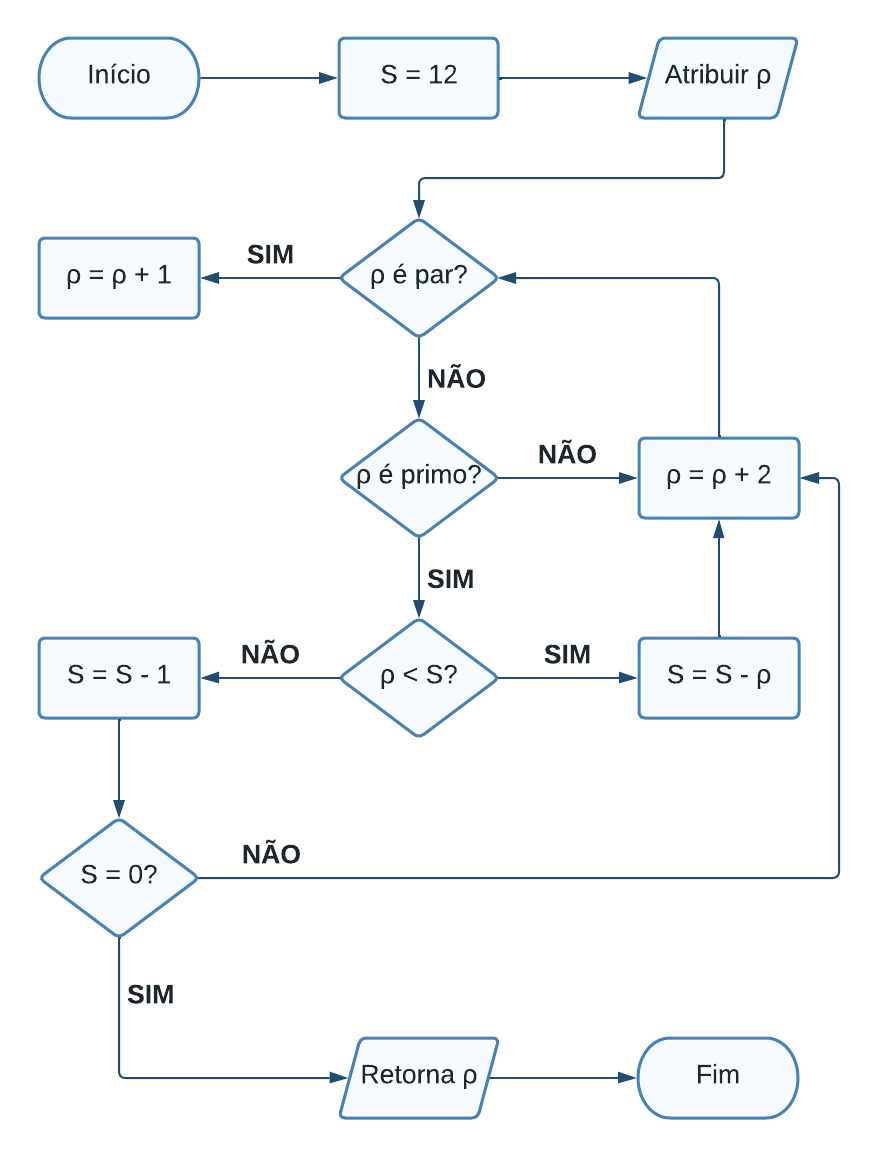
\includegraphics[width = \CaptionWidth]{fcht-ex-algorithm}
\SourceOrNote{autoria própria (\YearNum)}
\end{flowchart}

Como mostrado na \Cref{phot:pg-campus}, objetos flutuantes (ilustrações) podem adicionalmente receber um código QR (\ENLang*{Quick Response} ou Resposta Rápida) contendo: URL (\ENLang*{Uniform Resource Locator} ou Localizador Uniforme de Recursos) ou informações complementares.

\begin{photograph}[!htbp]
\SetCaptionWidth{\ifbool{@LayoutA}{0.6}{0.5}\linewidth}
\caption{Fachada do campus Ponta Grossa da UTFPR}%
\label{phot:pg-campus}
\savebox0{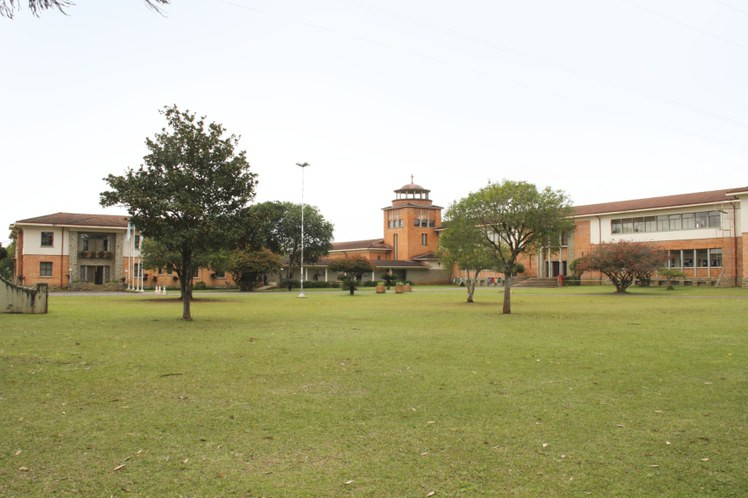
\includegraphics[width = \CaptionWidth]{phot-pg-campus}}
\usebox0%
\llap{%
  \raisebox{\ht0-\height}{%
    \href{https://www.utfpr.edu.br/campus/pontagrossa}{%
      
\includegraphics[height = 10mm]{phot-pg-campus-qr-code}%
    }%
  }%
}
\SourceOrNote{\textcite{UTFPR2018}}
\end{photograph}

O \Cref{grph:t-x} foi produzido usando o ambiente \LaTeX\ \texttt{tikzpicture} do pacote \LaTeX\ \texttt{tikz} a partir do arquivo \texttt{grph-t-x.tex} em \texttt{./Figures/}.

\begin{graph}[!htbp]
\SetCaptionWidth{\ifbool{@LayoutA}{0.7}{0.6}\linewidth}
\caption{Exemplo de gráfico}%
\label{grph:t-x}
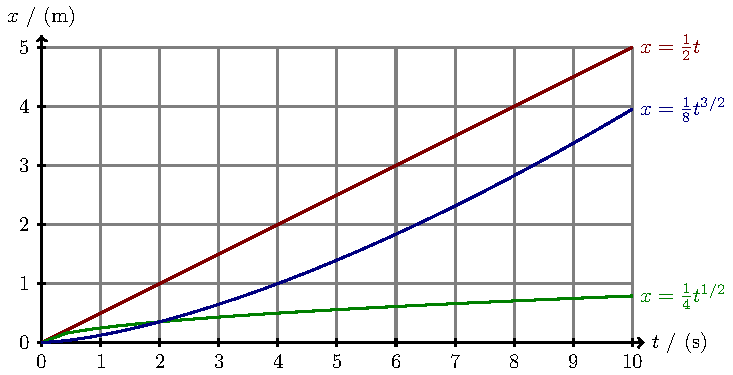
\includegraphics[width = \CaptionWidth]{grph-t-x}
\SourceOrNote{autoria própria (\YearNum)}
\end{graph}

Quadros devem ser inseridos seguindo a estrutura demonstrada no \Cref{tfrm:typography}.
Caso os dados sejam inéditos e provenientes de uma pesquisa realizada pelos próprios autores do trabalho, essa especificação deve constar na fonte com o ano da pesquisa de campo, por exemplo: autoria própria (\YearNum).

\begin{tabframed}[!htbp]
\caption{Tipografia dos títulos de seções}%
\label{tfrm:typography}
\begin{tabularx}{\linewidth}{?{}X|X?{}}%% CHKTEX 44
\toprule%
\multicolumn{1}{?{}Y|}{\textbf{Com numeração de seções}} &
\multicolumn{1}{Y?{}}{\textbf{Sem numeração de seções}}  \\ \midrule%
\textbf{1 TÍTULO DE SEÇÃO PRIMÁRIA}          & \textbf{TÍTULO DE SEÇÃO PRIMÁRIA} \\ \midrule%
\textbf{1.1 Título de Seção Secundária}      & TÍTULO DE SEÇÃO SECUNDÁRIA        \\ \midrule%
\textbf{1.1.1 Título de Seção Terciária}     & Título de Seção Terciária         \\ \midrule%
\textbf{1.1.1.1 Título de seção quaternária} & Título de seção quaternária       \\ \midrule%
\textbf{1.1.1.1.1 Título de seção quinária}  & \textit{Título de seção quinária} \\ \bottomrule%
\end{tabularx}
\SourceOrNote{autoria própria (\YearNum)}
\end{tabframed}

\subsection{Tabelas}%
\label{ssect:tab}

Assim como quadros, tabelas devem estar centralizadas e conter apenas dados imprescindíveis, não repetindo dados já inseridos no texto, ou vice-versa, evitando-se que sejam muito extensas.
O formato de tabela pode ser observado na \Cref{tab:example}.

\begin{table}[!htbp]
\SetCaptionWidth{0.5\linewidth}
\caption{Exemplo de tabela}%
\label{tab:example}
\begin{tabularx}{\CaptionWidth}{@{}XY@{}}
\toprule%
\multicolumn{1}{Y}{\textbf{Idade}}           &
\multicolumn{1}{Y}{\textbf{Percentual (\%)}} \\ \midrule%
Até 20 anos     & 0  \\
De 21 a 30 anos & 10 \\
De 31 a 40 anos & 20 \\
De 41 a 50 anos & 30 \\ \bottomrule%
\end{tabularx}
\SourceOrNote{adaptada de \textcite{Beltrano2021}}
\end{table}

Tabelas podem ser inseridas usando o ambiente \LaTeX\index{TeX@\TeX!LaTeX@\LaTeX} \texttt{table}, conforme exemplo no arquivo-fonte deste modelo.
Diversas ferramentas podem ser usadas para gerar ou editar tabelas em \LaTeX\index{TeX@\TeX!LaTeX@\LaTeX}, por exemplo: \ENLang{\href{https://www.tablesgenerator.com/}{Tables Generator\LinkIcon} e \href{https://www.latex-tables.com/}{\LaTeX\index{TeX@\TeX!LaTeX@\LaTeX} Tables Editor\LinkIcon}}.

\section{Conclusões}%
\label{sect:concl}

As conclusões ou considerações finais podem ser apresentadas como uma lista de itens, enfatizando as contribuições do trabalho:

\begin{itemize}
\item Primeiro item de conclusão.
\item Segundo item de conclusão.
\item Terceiro item de conclusão.
\item Quarto item de conclusão.
\item Quinto item de conclusão.
\end{itemize}

\ifbool{@LayoutA}{%
  \section*{Agradecimentos}[sect:ack]

  Seção obrigatória em trabalhos que receberam bolsa ou auxílio financeiro.
  Deve apresentar os agradecimentos aos principais órgãos de fomento (bolsa ou auxílio financeiro), instituições e pessoas que contribuíram para a realização do trabalho.
  Não exceder 50 palavras.
}{%
  \begin{InfoSection}{Agradecimentos}
  Seção obrigatória que serve para agradecer instituições e pessoas que contribuíram para a realização do trabalho, especialmente órgãos de fomento que viabilizaram recursos no formato de bolsa e auxílio financeiro.
  \end{InfoSection}

  \begin{InfoSection}{Material suplementar}
  Seção opcional que serve para informar ao leitor se há algum material suplementar ao trabalho e onde o mesmo pode ser obtido.
  Do contrário, remover.
  \end{InfoSection}

  \begin{InfoSection}{Disponibilidade de código}
  Seção opcional que serve para declarar se algum código desenvolvido está disponível para terceiros, explicitando onde o mesmo pode ser obtido.
  Do contrário, explicitar a razão para a indisponibilidade.
  Remover caso nenhum código tenha sido desenvolvido.
  \end{InfoSection}

  \begin{InfoSection}{Conflito de interesse}
  Seção obrigatória que serve para os autores declararem se possuem ou não algum conflito de interesse.
  Não havendo, sugere-se declarar \enquote{Não há conflito de interesse}.
  \end{InfoSection}

%   \begin{InfoSection}{Objetivos de Desenvolvimento Sustentável (ODS)}
%   Este trabalho pretende contribuir nos seguintes Objetivos de Desenvolvimento Sustentável (ODS):\\%
%   \parbox[t][0.75\BottomLine+0.5\baselineskip][c]{\linewidth}{\PrintSDGStamps[\baselineskip]}
%   \end{InfoSection}
}

\printbibliography%% Referências

%% Elementos pós-textuais (opcionais)
%% Editar o {Arquivo} para alterar: Glossário, Apêndices, Anexos e Índice
%% Remissivo.
% %%%% Elementos pós-textuais (opcionais)
%%
%% Glossário, Apêndices, Anexos e Índice Remissivo.

%% Glossário (inserir itens em ordem alfabética)
\begin{Glossary}%[\bfseries]%% Estilo do termo (item)
\item[Bib\LaTeX] reimplementação completa das facilidades bibliográficas fornecidas pelo \LaTeX.
\item[Bib\TeX] aplicativo de gerenciamento de referências para a formatação de listas de referências no \LaTeX.
\item[GEDWeb] sistema desenvolvido para gerenciar grandes acervos de normas e informações técnicas.
\item[ID Lattes] sequência de 16 dígitos que permite que qualquer pessoa encontre o Currículo Lattes de um{(a)} pesquisador{(a)}.
\item[\LaTeX] conjunto de macros para o processador de textos \TeX, utilizado amplamente para a produção de textos matemáticos e científicos devido à sua alta qualidade tipográfica.
\item[ORCID] código alfanumérico não proprietário para identificar exclusivamente cientistas, outros autores acadêmicos e contribuidores (\ENLang*{Open Researcher and Contributor ID} ou ID Aberto de Pesquisador e Contribuidor).
\item[\TeX] sistema de tipografia criado por Donald E. Knuth.
\item[\UTFPR-Article] modelo \LaTeX\ (não oficial) que permite a produção de artigos da Universidade Tecnológica Federal do Paraná (UTFPR), inclusive para eventos.
\end{Glossary}

%% Apêndices
\begin{Appendix}

\section{Título de Apêndice}%
\label{sect:apx-a1}

Exemplo de apêndice (\Cref{sect:apx-a1}) em uma seção de \nameref{sect:appendix}.

\subsection{Título de Seção Secundária de Apêndice}%
\label{ssect:apx-a2}

Exemplo de seção secundária de apêndice (\Cref{ssect:apx-a2}).

\subsubsection{Título de Seção Terciária de Apêndice}%
\label{sssect:apx-a3}

Exemplo de seção terciária de apêndice (\Cref{sssect:apx-a3}).

\paragraph{Título de seção quaternária de Apêndice}%
\label{prgh:apx-a4}

Exemplo de seção quaternária de apêndice (\Cref{prgh:apx-a4}).

\subparagraph{Título de seção quinária de Apêndice}%
\label{sprgh:apx-a5}

Exemplo de seção quinária de apêndice (\Cref{sprgh:apx-a5}).

\end{Appendix}

%% Anexos
\begin{Annex}

\section{Título de Anexo}%
\label{sect:anx-a1}

Exemplo de anexo (\Cref{sect:anx-a1}) em uma seção de \nameref{sect:annex}.

\subsection{Título de Seção Secundária de Anexo}%
\label{ssect:anx-a2}

Exemplo de seção secundária de anexo (\Cref{ssect:anx-a2}).

\subsubsection{Título de Seção Terciária de Anexo}%
\label{sssect:anx-a3}

Exemplo de seção terciária de anexo (\Cref{sssect:anx-a3}).

\paragraph{Título de seção quaternária de Anexo}%
\label{prgh:anx-a4}

Exemplo de seção quaternária de anexo (\Cref{prgh:anx-a4}).

\subparagraph{Título de seção quinária de Anexo}%
\label{sprgh:anx-a5}

Exemplo de seção quinária de anexo (\Cref{sprgh:anx-a5}).

\end{Annex}

%% Índice Remissivo
\printindex%


%% Fim do documento
\end{document}
